%!TEX root = practicum3.tex
To measure the performance of the SGD algorithm, we split the available data into two data sets. The first set we use to train the algorithm and the other to test its performance. 

To measure the performance while learning, the learning rate of the SGD algorithm can be calculated using the error (the cost function from \eqref{eq:1:cost}) on the training data set. The performance of the algorithm on unseen data, the generalization error, can be measured using the same error function on the test data set. Both errors are computed after every epoch $t$ and thus after every $P$ training steps. The two curves are shown in \cref{fig:exp:errors}.

\begin{figure}
	\centering
	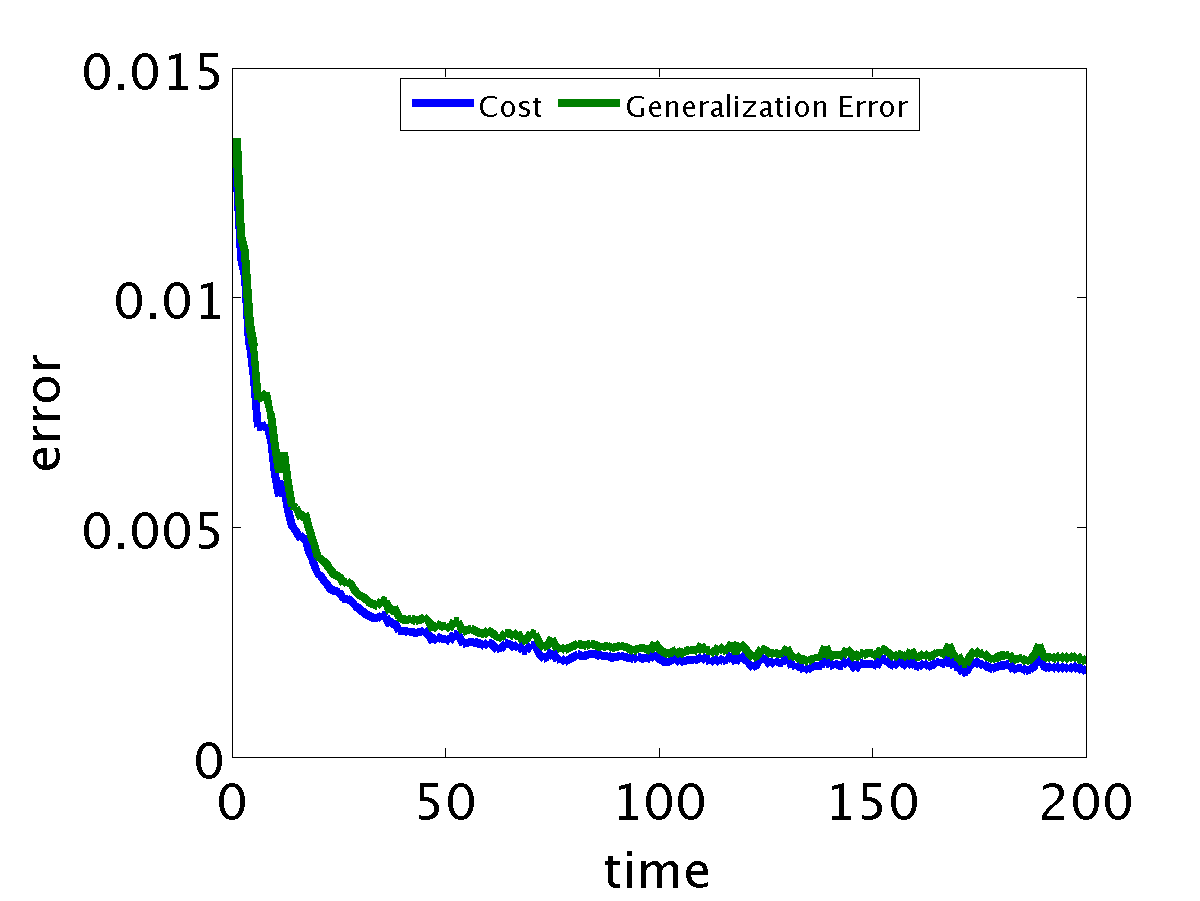
\includegraphics[width=\columnwidth]{./img/errors_train_2000_test_2000.png}
	\caption{The cost, shown in blue, and the generalization error, shown in green, of a training set and test set with each 2000, 50-dimensional points for each epoch, with $t_{max} = 200$, $\eta = 0.05$.}
	\label{fig:exp:errors}
\end{figure}

One would expect that the error on the training data would be lower than on the test data, because the network is trained specifically on the data from that training data set. One can observe this difference between the two errors in \cref{fig:exp:errors}.

\begin{figure}
	\centering
	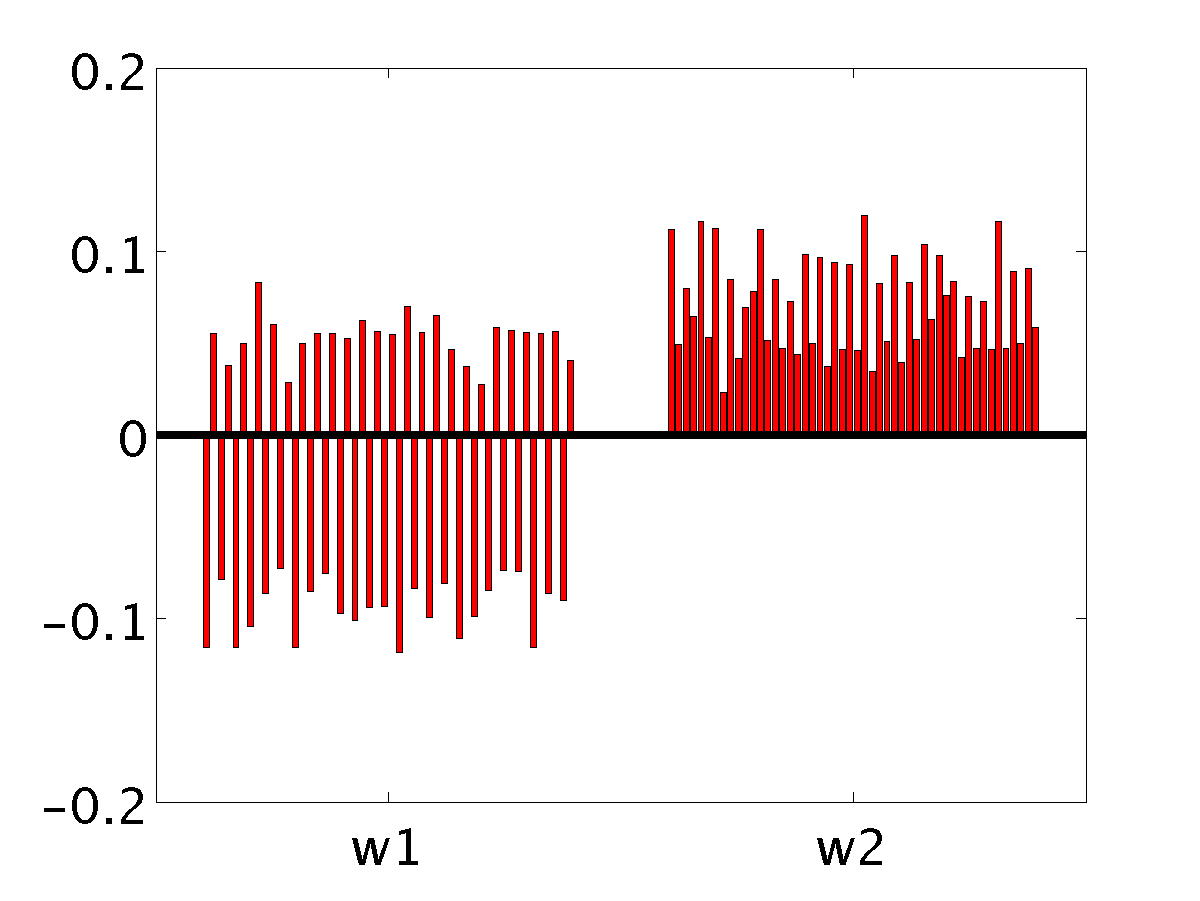
\includegraphics[width=\columnwidth]{./img/weights_train_2000_test_2000.png}
	\caption{The values of the elements of the two weights vectors at $t = 200$.}
	\label{fig:exp:weights}
\end{figure}